\documentclass{article}

\usepackage{multicol}
\usepackage{authblk}
\usepackage{blindtext}
\usepackage{graphicx}
\usepackage{booktabs}
\usepackage{placeins}
\usepackage{siunitx}
\usepackage[a4paper, total={6.5in, 10in}]{geometry}
\usepackage[colorlinks,citecolor=blue,urlcolor=red,bookmarks=false,hypertexnames=true]{hyperref}
\usepackage{amsmath}
\usepackage{academicons}
\usepackage{xcolor}

%\graphicspath{ {imgs/} }

\newbox{\myorcidaffilbox}
\sbox{\myorcidaffilbox}{\large
\includegraphics[height=1.7ex]{imgs/ORCIDiD_icon16x16.png}}

\newcommand{\orcidaffil}[1]{%
	\href{https://orcid.org/#1}{\usebox{\myorcidaffilbox}}}

\newcommand{\showorcidaffil}[1]{%
	\href{https://orcid.org/#1}{\usebox{\myorcidaffilbox}}#1}

\newcommand{\icol}[1]{% inline column vector
	\left(\begin{bmatrix}#1\end{bmatrix}\right)%
}

\newcommand{\irow}[1]{% inline row vector
	\begin{bmatrix}#1\end{bmatrix}%
} 


\author[1]{Quang Huy Pham \orcidaffil{0000-0000-0000-0000}}
\author[1]{Hoang Khoi Do \orcidaffil{0000-0000-0000-0000}}
\author[2]{Lan Dang Hoang \orcidaffil{0000-0000-0000-0000}}
\affil[1]{Author Affiliation1}
\affil[2]{Author Affiliation2}
\affil[ ]{\textit {\{huy.pq200282, khoi.dh200332, lan.dh203810\}@sis.hust.edu.vn}}

\begin{document}
	\title{Digital Communication System on Gaussion Noise using QPSK modulation and LDPC}	
	
	\maketitle
	
	\begin{abstract}
		
	\end{abstract}
	
	\section{Introduction}
	
	In the era of digital technology, telecommunication plays an important role of data transaction, wireless communication. There has been many wireless communication application, technique research recently to bring the most applicable solution to increase the experience on using service. In 5G system, the latency of data transmission is 1ms compared to 10ms of 4G system. This result is achieve owing to the various high deep technologies integrated into 5G wireless communication system. One of those top-notch technologies is Low-Density Parity-Check codes (LDPC).
	
	The Noisy Channel Coding Theorem discovered by C.E. Shannon in 1948 offered communication engineers the possibility of reducing error rates on noisy channels to negligible levels without sacrificing data rates. The primary obstacle to the practical use of this theorem has been the equipment complexity  and the computation time required to decode the noisy received data. Channel coding is a technique achieving high data rates and negligible error probabilities on noisy channels with a reasonable amount of equipment. The pros and cons of this technique over other techniques for the same prupose are neither simple nor clear-cut, and depend primarily upon the channel and the type of service required. More important than the particular technique, however, is the hope that the concepts here will lead to new and better coding procedure.
	
	Low-density parity-check codes (LDPC codes) are efficient channel coding codes
	that allow transmission errors to be corrected. They were first described in 1960 by	Gallager in his dissertation \cite{Gal63}. These codes did not gain general acceptance, not	least because of the computational effort required to calculate them, and they were forgotten again.	Prompted by the groundbreaking development of Turbo codes by Berrou, Glavieux and Thitimajshima \cite{Ber93}, which allow coding close to the channel capacity predicted by Claude E. Shannon \cite{Sha48}, LDPC codes have been rediscovered \cite{Mac96}.
	
	In this report, a comparison between the performance of LDPC and several channel coding techniques is conducted by using simulation. White noise, on the other hand is also considered as noise in experiment. 
	
	\section{Materials and Methodology}
	\subsection{Material}
	In order to conduct the simulation Matlab 2018b is used. The environment used for Matlab is Ubuntu 20.04. 
	\subsection{Methodology} 
	\subsubsection{LDPC coding}
	\subsubsection{QPSK modulation}
	The Quadrature Phase Shift Keying(QPSK) is a variation of BPSK, and it is also a Double Side Band Suppressed Carrier DSBSC modulation scheme, which sends two bits of digital information at a time, called as bigits. Instead of the conversion of digital bits into a series of digital stream, it converts them into bit pairs. This decreases the data bit rate to half, which allows space for the other users.
	
	The QPSK Modulator uses a bit-splitter, two multipliers with local oscillator, a 2-bit serial to parallel converter, and a summer circuit (see Figure \ref{fig:qpsk_mo}). 
	
	\begin{figure}[h]
		\caption{QPSK Modulation}
		\centering
		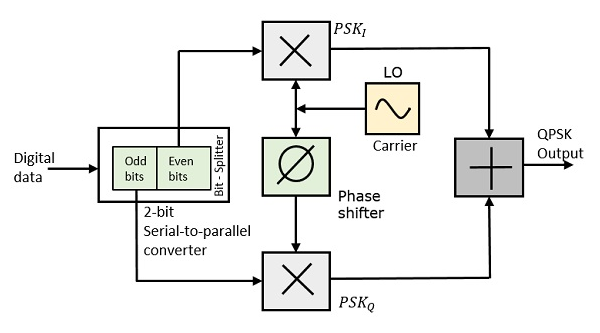
\includegraphics[width=0.6\textwidth]{imgs/qpsk_modulator}
		\label{fig:qpsk_mo}
	\end{figure}

	At the modulator’s input, the message signal’s even bits (i.e., $2^{nd}$ bit, $4^{th}$ bit, $6^{th}$ bit, etc.) and odd bits (i.e., $1^{st}$ bit, $3^{rd}$ bit, $5^{th}$ bit, etc.) are separated by the bits splitter and are multiplied with the same carrier to generate odd BPSK (called as $PSK_I$) and even BPSK (called as $PSK_Q$). The $PSK_Q$ signal is anyhow phase shifted by 90° before being modulated. The QPSK waveform for two-bits input is shown in Figure \ref{fig:qpsk_mo_show}. 
	
	\begin{figure}[h]
		\caption{QPSK Waveform}
		\centering
		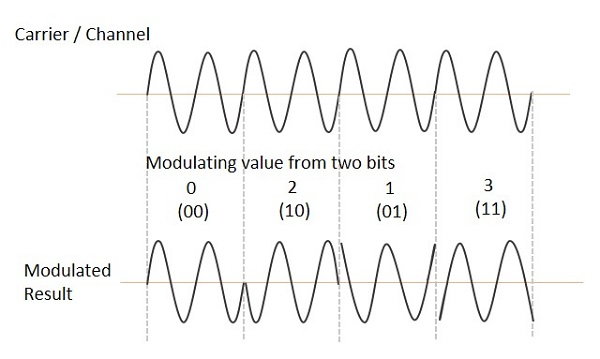
\includegraphics[width=0.6\textwidth]{imgs/qpsk_waveform}
		\label{fig:qpsk_mo_show}
	\end{figure}
	
	On the other hand, the QPSK Demodulator uses two product demodulator circuits with local oscillator, two band pass filters, two integrator circuits, and a 2-bit parallel to serial converter (see Figure \ref{fig:qpsk_demo}).
	
	\begin{figure}[h]
		\caption{QPSK Waveform}
		\centering
		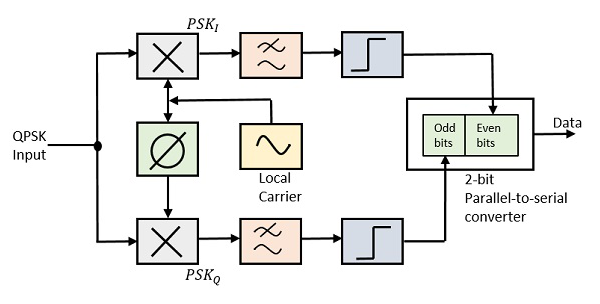
\includegraphics[width=0.6\textwidth]{imgs/qpsk_demodulator}
		\label{fig:qpsk_demo}
	\end{figure}

	The two product detectors at the input of demodulator simultaneously demodulate the two BPSK signals. The pair of bits are recovered here from the original data. These signals after processing, are passed to the parallel to serial converter.

	\subsubsection{AWGN Channel}
	\textbf{Additive white Gaussian noise (AWGN)} is a basic noise model used in information theory to mimic the effect of many random processes that occur in nature. The modifiers denote specific characteristics:
	\begin{itemize}
		\item \textbf{Additive} because it is added to any noise that might be intrinsic to the information system.
		\item \textbf{White} refers to the idea that it has uniform power across the frequency band for the information system. It is an analogy to the color white which has uniform emissions at all frequencies in the visible spectrum.s
		\item \textbf{Gaussian} because it has a normal distribution in the time domain with an average time domain value of zero.
	\end{itemize}
	The AWGN channel is represented by a series of outputs $Y_i$ at discrete time event index $i$. $Y_i$ is the sum of the input $X_i$ and noise, $Z_i$ (see Equation \ref{eq:awgn}), where $Z_i$ is independent and identically distributed and drawn from a zero-mean normal distribution with variance $N$. The $Z_i$ are further assumed to not be correlated with the $X_i$.
	\begin{equation}
		 Y_i = X_i + Z_i \quad \textrm{where} \quad Z_i \sim N(0, N)
		 \label{eq:awgn}
	\end{equation}
	\section{Results}
	\section{Conclusion}
	
	%Biliography Rendering
	\bibliographystyle{ieeetr} 
	\bibliography{ref} 
	
	%Appendix Starting
	\appendix

\end{document}



